\documentclass[11pt]{article}
\usepackage[utf8]{inputenc}
\usepackage[english]{babel}
\usepackage[
backend=biber,
style=alphabetic,
sorting=ynt
]{biblatex}
\addbibresource{references.bib}
\usepackage{amsmath}  % Basic math symbols and environments
\usepackage{amssymb}  % Extended symbol collection
\usepackage{mathtools} % Fixes and additions to amsmath
\usepackage{graphicx}
\usepackage{float}
\usepackage{csvsimple}
\usepackage[colorlinks=true]{hyperref}
\usepackage{indentfirst}
\usepackage{algorithm}
\usepackage{algpseudocode}
\DeclareGraphicsExtensions{.png,.pdf}
\begin{document}

\noindent
\textbf{title:} AIML429 - Portfolio 2 \\
\textbf{date:} May 29, 2026 \\
\textbf{author:} Jason Pollock \\
\textbf{email:} jason@pollock.ca, pollocjaso@myvuw.ac.nz \\
	
\section{Rejection Sampling}

\subsection{a - plots}

% Wolfram equation:
% {e^(-x^(2)/2)* (2 + sin(3 x + 1)), (1/(sqrt(2pi)))*e^(-x^2/2)} 

\begin{align}
	q(x) &= N(x;0,1) \\
	&= 1/(\sigma \sqrt{2 \pi}) * e^{-1/2*((x-\mu)/\sigma)^2} \\
	&= 1/(\sqrt(2 \pi)) * e^{-x^2/2}
\end{align}

An exact solution for C is possible:

\begin{align}
	q(x) &= 1/(\sqrt(2 \pi)) * e^{-x^2/2}  \\
	p(x) &= e^{-x^{2}/2}* (2 + sin(3 x + 1)) \\
	q(x) & >= p(x) \\
	1/(\sqrt(2 \pi)) * e^{-x^2/2} &>= e^{-x^{2}/2}* (2 + sin(3 x + 1)) \\
	c &>= \sqrt{2 \pi} * (2 + sin(3x+1)) \\
	c &>= \sqrt{2 \pi} * (2 + 1) \\
	c &>= 3 \sqrt{2\pi}
\end{align}

\begin{figure}[H]
	\centering
	\begin{minipage}{.6\textwidth}
		\centering
		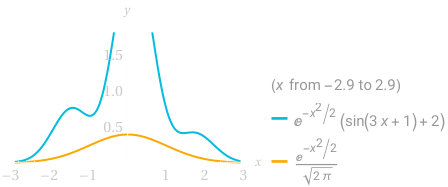
\includegraphics[width=1.0\textwidth]{rejection_c_1}
		\caption{c = 1}
		\label{fig:1.1}
	\end{minipage}%
	\begin{minipage}{.6\textwidth}
		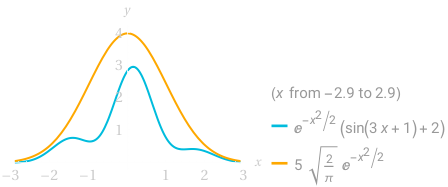
\includegraphics[width=1.0\textwidth]{rejection_c_10}
		\caption{c = 10}
		\label{fig:1.2}
	\end{minipage}
	\begin{minipage}{.6\textwidth}
		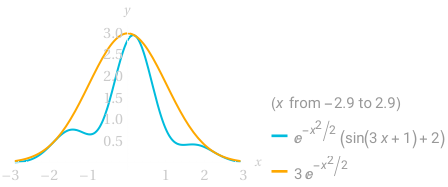
\includegraphics[width=1.0\textwidth]{rejection_c_3pi}
		\caption{c = $(3 * \sqrt{2 \pi})$}
		\label{fig:1.3}
	\end{minipage}
\end{figure}



\subsection{b - sigma = 100}

% Wolfram equation
%{e^(-x^(2)/2)* (2 + sin(3 x + 1)),1/(100*sqrt(2pi)) * e^(-1/2*(x/100)^2)} 

\begin{figure}[H]
	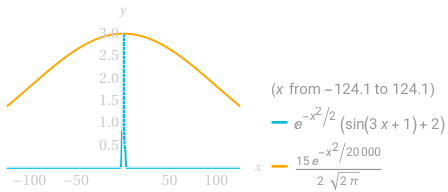
\includegraphics[width=1.0\textwidth]{rejection_sigma_100_c_750}
	\caption{ $(c = 750)$, $(\sigma = 100)$}
	\label{fig:3.i.a}
\end{figure}

C has to increase substantially to bring the peak probability up to the other equation. This is because the probability is spread over a much larger area. Since the area between the two curves is a lot larger, the sample acceptance rate will decrease dramatically.

While N(0,1) seems very similar to p(x) from x = 5, N(0,100) has a wide band, even out past x = +- 100.


\subsection{c - expectation}

See sampling.ipnyb.

The expectation was measured as 0.57. Since Option 1 has a fixed payout of 1, it has a higher expectated value and should be preferred.

\section{Metroplis-Hastings by hand}

\subsection{acceptance probability, simplified}
\begin{align}
	Accept(x->x') &= min(1,\propto) \\
	\propto &= \frac{p(x')}{p(x)} \frac{q(x|x')}{q(x'|x)}
\end{align}
Since q is the normal distribution,
\begin{align}
	q(x|x') &= q(x'|x)\\
	\propto &= \frac{p(x')}{p(x)} \\
	Accept(x->x') &= min(1,\frac{p(x')}{p(x)}) \\
\end{align}

\subsection{Compute $\propto$'s}

\begin{align}
	\propto(A->B) &= \frac{\Pi(B)}{\Pi(A)} = \frac{\frac{3}{10}}{\frac{5}{10}} = 3/5 \\
	\propto(A->C) &= \frac{\Pi(C)}{\Pi(A)} = \frac{\frac{2}{10}}{\frac{5}{10}} = 2/5 \\	
	\propto(B->A) &= \frac{\Pi(A)}{\Pi(B)} = \frac{\frac{5}{10}}{\frac{3}{10}} = 5/3 \\		
\end{align}

\subsection{Trace the chain}

\begin{itemize}
	\item A-\textgreater B: $\frac{\Pi(B)}{\Pi(A)} = 3/5 >= 0.4$, Accept
	\item B-\textgreater C: $\frac{\Pi(C)}{\Pi(B)} = 2/3 !>= 0.8$, Reject
	\item B-\textgreater A: $\frac{\Pi(A)}{\Pi(B)} = 5/3 = 1$, Accept		
\end{itemize}

Final chain is A, B, A.

\subsection{Detailed Balance Proof}

The condition is detailed balance:
\begin{align}
	\frac{M_{x->x'}}{M_{x'->x}} &= \frac{\Pi(x')}{\Pi(x)} \\
	\frac{M_{x->x'}}{M_{x'->x}} &= \frac{Q_{x->x'} A_{x->x'}}{Q_{x'->x} A_{x'->x}} \\
	&= \frac{A_{x->x'}}{A_{x'->x}} \\
	\Pi(x') &= \Pi(B) = 3/10 \\
	\Pi(x) &= \Pi(A) = 5/10 \\
	 A_{x->x'} &= min(1, \frac{p(x')}{p(x)}) = min(1, (3/10)/(5/10)) = 3/5 \\
	 A_{x'->x} &= min(1, \frac{p(x)}{p(x')}) = min(1, (5/10)/(3/10)) = 1 \\
	 \frac{M_{x->x'}}{M_{x'->x}} &= \frac{A_{x->x'}}{A_{x'->x}} 
	 &= (3/5)/1 = 3/5
	 &=  \frac{\Pi(B)}{\Pi(A)} = (3/10)/(5/10) = 3/5
\end{align}

\section{About "flat" priors}

\subsection{flat where?}
\begin{figure}[H]
	\centering
	\begin{minipage}{.4\textwidth}
		\centering
		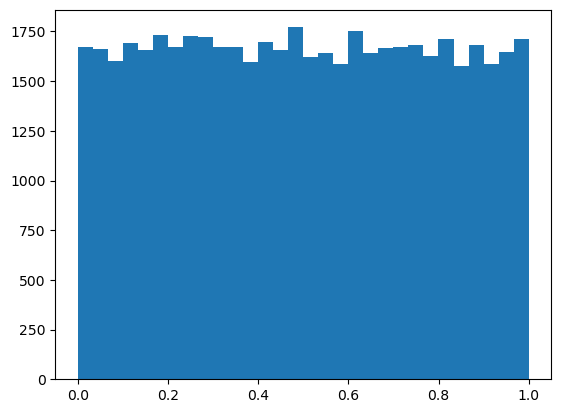
\includegraphics[width=1.0\textwidth]{beta_1_1}
		\caption{Beta(1,1)}
		\label{fig:3.1}
	\end{minipage}%
	\begin{minipage}{.4\textwidth}
		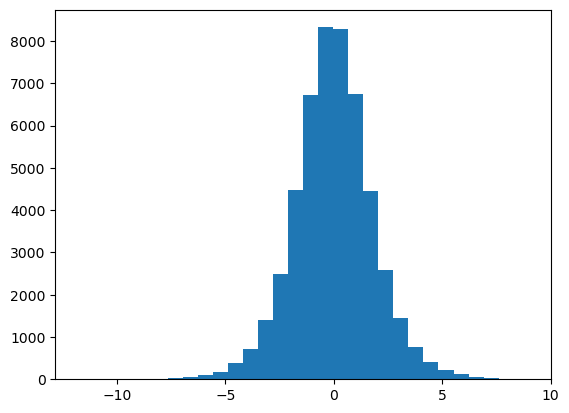
\includegraphics[width=1.0\textwidth]{beta_1_1_log}
		\caption{Beta(1,1) log-odds}
		\label{fig:3.2}
	\end{minipage}
	\begin{minipage}{.4\textwidth}
		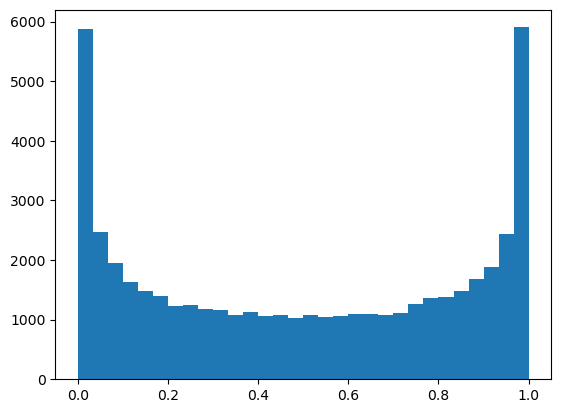
\includegraphics[width=1.0\textwidth]{beta_5_5}
		\caption{Beta(0.5, 0.5)}
		\label{fig:3.3}
	\end{minipage}
	\begin{minipage}{.4\textwidth}
		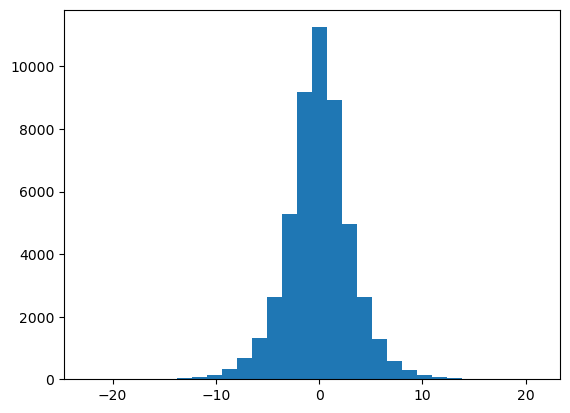
\includegraphics[width=1.0\textwidth]{beta_5_5_log}
		\caption{Beta(0.5, 0.5 log-odds}
		\label{fig:3.4}
	\end{minipage}	
\end{figure}

The Beta(1,1) distribution is flatter in $\theta$ space. The Beta(0.5, 0.5) distribution appears to have extremes at both ends of the distribution. However in log space, the Beta(0.5, 0.5) distribution is spread out more, with a higher peak as well.

It is strange that Beta(0.5, 0.5) has a solution, but Beta(0.1, 0.1) produces infinities.

\subsection{Small-data posteriors}

\begin{figure}[H]
	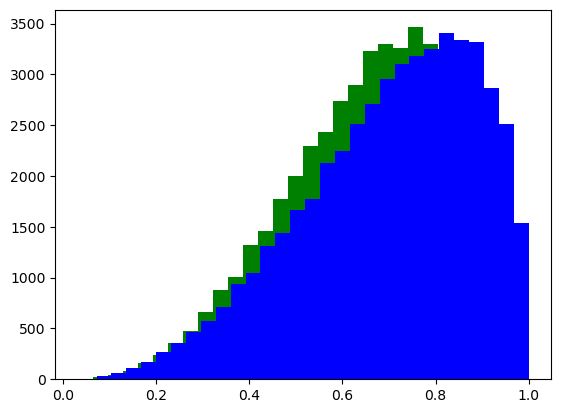
\includegraphics[width=1.0\textwidth]{posterior_coin}
	\caption{green=Beta(4,2), blue=Beta(3.5,1.5)}
	\label{fig:3.5}
\end{figure}

They differ most on how far to the left they've shifted. This makes intuitive sense. The Beta(1,1) distribution has more total coin "flips". At small numbers this will shift the mean noticeably.

The difference in the peak shows up in the mean - 4/6 = 20/30 vs 3.5/5 = 21/30.

\subsection{Large-data posteriors}

\begin{figure}[H]
	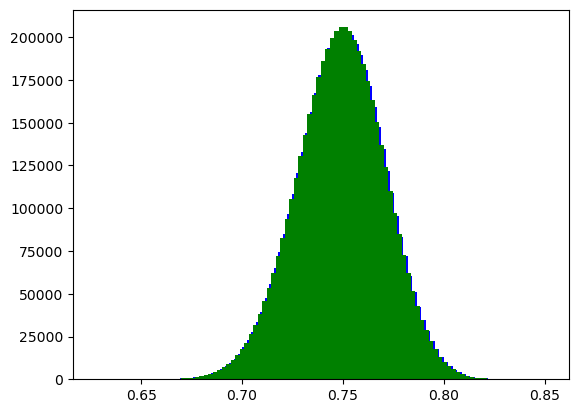
\includegraphics[width=1.0\textwidth]{posterior_coin_large_data}
	\caption{green=Beta(1,1), blue=Beta(0.5,0.5)}
	\label{fig:3.6}
\end{figure}

\section{naïve Bayes: when does Bayesian inference stay tractable?}

\section{Bayesian linear regression}

\section{Bayesian neural network via Metroplis sampling}

\section{sigmoids: generative vs. discriminative}

\section{EuroSCORE: upstream or downstream?}

\section{EuroSCORE: how are the parameters learnt?}

\section{KL divergence}

\section{ELBO}


	


\end{document}
